\documentclass{article}

\title{Paths}
\author{Natalie Weaver}

\usepackage{minted}  % Code formatting and highlighting
\usepackage{tikz}  % Tools for graphics creation

% Macros

% Abbreviations of common compound commands
\newcommand{\mlatex}[1] {
    \mintinline{latex}{#1}
}

\begin{document}

\maketitle
\tableofcontents

\section{Path definition}

A path is a series of coordinates; paths are the most basic building blocks of tikz pictures. We can define a path using the \mlatex{\path} command within a \mlatex{tikzpicture} environment. By default, nothing is drawn.

\begin{minted}{latex}
    \begin{tikzpicture}
        \path (0, 0) -- (1, 1) -- (-1, 2) -- cycle;
    \end{tikzpicture}
\end{minted}

\begin{tikzpicture}
    \path (0, 0) -- (1, 1) -- (-1, 2) -- cycle;
\end{tikzpicture}

\section{Actions}

To see the path, we can use the optional action argument, which takes one or more of the following values:

\begin{itemize}
    \item \mlatex{draw}
    \item \mlatex{fill}
    \item \mlatex{shade}
    \item \mlatex{clip}
\end{itemize}

Tikz comes with built-in abbreviations for commonly-used combinations of these values.

\subsection{Draw}

\mlatex{draw} simply draws the line segments of the path, and does not require the path to be closed.

\begin{minted}{latex}
    % Long form
    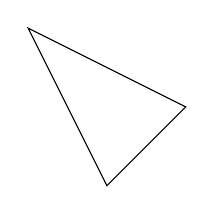
\begin{tikzpicture}
        \path[draw] (0, 0) -- (1, 1) -- (-1, 2) -- cycle;
    \end{tikzpicture}

    % Abbreviated form
    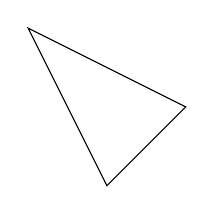
\begin{tikzpicture}
        \draw (0, 0) -- (1, 1) -- (-1, 2) -- cycle;
    \end{tikzpicture}
\end{minted}

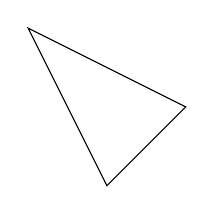
\begin{tikzpicture}
    \path[draw] (0, 0) -- (1, 1) -- (-1, 2) -- cycle;
\end{tikzpicture}

\begin{minted}{latex}
    \begin{tikzpicture}
        \draw (0, 0) -- (1, 1) -- (-1, 2);
    \end{tikzpicture}
\end{minted}

\begin{tikzpicture}
    \draw (0, 0) -- (1, 1) -- (-1, 2);
\end{tikzpicture}

\subsection{Fill}

\mlatex{fill} fills in the region enclosed by the path (which is required to be closed). If the path is not closed, tikz will automatically close it for us.

\begin{minted}{latex}
    % Long form
    
\begin{tikzpicture}
        \path[fill] (0, 0) -- (1, 1) -- (-1, 2) -- cycle;
    \end{tikzpicture}

    % Abbreviated form
    
\begin{tikzpicture}
        \fill (0, 0) -- (1, 1) -- (-1, 2) -- cycle;
    \end{tikzpicture}
\end{minted}


\begin{tikzpicture}
    \path[fill] (0, 0) -- (1, 1) -- (-1, 2) -- cycle;
\end{tikzpicture}

\begin{minted}{latex}
    
\begin{tikzpicture}
        \fill (0, 0) -- (1, 1) -- (-1, 2);
    \end{tikzpicture}
\end{minted}


\begin{tikzpicture}
    \fill (0, 0) -- (1, 1) -- (-1, 2);
\end{tikzpicture}

\subsection{Shade}

\mlatex{shade} shades the region enclosed by the path (which is required to be closed). If the path is not closed, tikz will automatically close it for us.

\begin{minted}{latex}
    % Long form
    
\begin{tikzpicture}
        \path[shade] (0, 0) -- (1, 1) -- (-1, 2) -- cycle;
    \end{tikzpicture}

    % Abbreviated form
    
\begin{tikzpicture}
        \shade (0, 0) -- (1, 1) -- (-1, 2);
    \end{tikzpicture}
\end{minted}


\begin{tikzpicture}
    \shade (0, 0) -- (1, 1) -- (-1, 2);
\end{tikzpicture}

\subsection{Clip}

\mlatex{clip} defines the region where graphics are permitted to appear. Only graphics located inside of the (closed) path are drawn. Note that tikz statements are executed sequentially, so the \mlatex{clip} command will only apply to statements below it.

\begin{minted}{latex}
    % Long form
    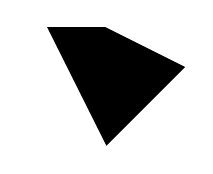
\begin{tikzpicture}
        \path[clip] (-1, 0) -- (1, 0) -- (1, 1.5) -- (-1, 1.5) -- cycle;
        \path[fill] (0, 0) -- (1, 1) -- (-1, 2) -- cycle;
    \end{tikzpicture}

    % Abbreviated form
    
\begin{tikzpicture}
        \clip (-1, 0) -- (1, 0) -- (1, 1.5) -- (-1, 1.5);
        \shade (0, 0) -- (1, 1) -- (-1, 2);
    \end{tikzpicture}
\end{minted}


\begin{tikzpicture}
    \clip (-1, 0) -- (1, 0) -- (1, 1.5) -- (-1, 1.5);
    \shade (0, 0) -- (1, 1) -- (-1, 2);
\end{tikzpicture}

\subsection{Aliased combinations}

\end{document}